\documentclass{beamer}
\usetheme{Madrid}
\usecolortheme{default}

\usepackage[utf8]{inputenc}
\usepackage[romanian]{babel}
\usepackage{amsmath}
\usepackage{amsfonts}
\usepackage{amssymb}
\usepackage{graphicx}
\usepackage{listings}
\usepackage{xcolor}
\usepackage{tikz}
\usetikzlibrary{shapes,arrows,positioning}

\title{Sistem Radar pentru Detecția Aeronavelor}
\subtitle{Analiză în Frecvență și Procesare Digitală}
\author{Ingrid Corobana}
\institute{An III - Prelucrarea Semnalelor}
\date{Decembrie 2025}

\begin{document}

\frame{\titlepage}

\begin{frame}{Cuprins}
\tableofcontents
\end{frame}

\section{Introducere}

\begin{frame}{Motivație}
\begin{block}{De ce un sistem radar?}
\begin{itemize}
    \item Creșterea traficului aerian
    \item Necesitatea monitorizării în timp real
    \item Siguranța aviației civile și militare
    \item Detecția dronelor și UAV-urilor
\end{itemize}
\end{block}

\begin{alertblock}{Provocări}
\begin{itemize}
    \item Detecție precisă la distanțe mari
    \item Zgomot și interferențe
    \item Ținte multiple simultane
    \item Costuri de implementare
\end{itemize}
\end{alertblock}
\end{frame}

\begin{frame}{Obiective Proiect}
\begin{enumerate}
    \item \textbf{Proiectare}: Sistem radar FMCW funcțional
    \item \textbf{Implementare}: Algoritmi de procesare în frecvență
    \item \textbf{Detectare}: Identificare și tracking ținte
    \item \textbf{Validare}: Teste și simulări extensive
\end{enumerate}

\vspace{0.5cm}

\begin{block}{Contribuții}
\begin{itemize}
    \item Simulator radar complet în Python
    \item Procesare avansată FFT cu CFAR
    \item Tracking multi-țintă
    \item Vizualizări interactive
\end{itemize}
\end{block}
\end{frame}

\section{Fundamentare Teoretică}

\begin{frame}{Principiul Radar FMCW}
\begin{columns}
\column{0.5\textwidth}
\textbf{FMCW} = Frequency Modulated Continuous Wave

\vspace{0.3cm}

\textbf{Caracteristici:}
\begin{itemize}
    \item Emisie continuă
    \item Frecvență variabilă (chirp)
    \item Putere redusă
    \item Cost eficient
\end{itemize}

\column{0.5\textwidth}
\begin{equation*}
s_{TX}(t) = A e^{j2\pi(f_c t + \frac{1}{2}kt^2)}
\end{equation*}

unde:
\begin{itemize}
    \item $f_c$ = frecvența purtătoare
    \item $k = B/T$ = chirp rate
    \item $B$ = bandwidth
    \item $T$ = timp sweep
\end{itemize}
\end{columns}
\end{frame}

\begin{frame}{Estimarea Distanței}
\begin{block}{Principiu}
Diferența de frecvență (beat frequency) dintre TX și RX → distanță
\end{block}

\begin{equation*}
\boxed{R = \frac{f_{beat} \cdot c \cdot T}{2B}}
\end{equation*}

\vspace{0.3cm}

\textbf{Exemplu:}
\begin{itemize}
    \item $f_{beat} = 33.3$ kHz
    \item $B = 100$ MHz, $T = 1$ ms
    \item $c = 3 \times 10^8$ m/s
    \item $\Rightarrow R = 5$ km
\end{itemize}
\end{frame}

\begin{frame}{Efectul Doppler}
Pentru ținte în mișcare:

\begin{equation*}
f_D = \frac{2v}{\lambda} = \frac{2vf_c}{c}
\end{equation*}

\vspace{0.5cm}

\begin{columns}
\column{0.5\textwidth}
\textbf{Apropiere:}
\begin{equation*}
f_{obs} = f_{beat} + f_D
\end{equation*}

\column{0.5\textwidth}
\textbf{Îndepărtare:}
\begin{equation*}
f_{obs} = f_{beat} - f_D
\end{equation*}
\end{columns}

\vspace{0.5cm}

\begin{exampleblock}{Viteză din Doppler}
\begin{equation*}
v = \frac{f_D \cdot \lambda}{2}
\end{equation*}
\end{exampleblock}
\end{frame}

\begin{frame}{Ecuația Radar}
Puterea recepționată:

\begin{equation*}
P_{RX} = \frac{P_{TX} \cdot G^2 \cdot \lambda^2 \cdot \sigma}{(4\pi)^3 \cdot R^4}
\end{equation*}

\vspace{0.3cm}

\textbf{Observații:}
\begin{itemize}
    \item Dependență $R^{-4}$ (atenuare rapidă!)
    \item RCS ($\sigma$) crucial pentru detectare
    \item SNR trebuie > 10 dB pentru detecție fiabilă
\end{itemize}

\vspace{0.3cm}

\begin{table}
\centering
\begin{tabular}{|l|c|}
\hline
\textbf{Tip aeronavă} & \textbf{RCS tipic} \\
\hline
Dronă mică & 0.1 - 1 m² \\
Elicopter & 2 - 10 m² \\
Avion comercial & 20 - 100 m² \\
\hline
\end{tabular}
\end{table}
\end{frame}

\section{Procesare în Frecvență}

\begin{frame}{Transformata Fourier Rapidă (FFT)}
\begin{block}{Definiție DFT}
\begin{equation*}
X[k] = \sum_{n=0}^{N-1} x[n] \cdot e^{-j2\pi kn/N}
\end{equation*}
\end{block}

\textbf{Complexitate:}
\begin{itemize}
    \item DFT directă: $O(N^2)$
    \item FFT (Cooley-Tukey): $O(N \log N)$
\end{itemize}

\vspace{0.3cm}

\textbf{Pentru $N = 4096$:}
\begin{itemize}
    \item DFT: $\sim 16$ milioane operații
    \item FFT: $\sim 49,000$ operații
    \item \textcolor{red}{Speedup: 330×!}
\end{itemize}
\end{frame}

\begin{frame}{Windowing pentru FFT}
\textbf{Problemă:} Leakage spectral

\textbf{Soluție:} Ferestre de ponderare

\vspace{0.3cm}

\begin{columns}
\column{0.5\textwidth}
\textbf{Fereastra Hamming:}
\begin{equation*}
w[n] = 0.54 - 0.46\cos\left(\frac{2\pi n}{N-1}\right)
\end{equation*}

\column{0.5\textwidth}
\textbf{Aplicare:}
\begin{equation*}
x_w[n] = x[n] \cdot w[n]
\end{equation*}
\end{columns}

\vspace{0.5cm}

\begin{alertblock}{Trade-off}
\begin{itemize}
    \item[+] Reducere leakage
    \item[-] Rezoluție ușor redusă
    \item[-] Pierdere în SNR ($\sim 1.4$ dB pentru Hamming)
\end{itemize}
\end{alertblock}
\end{frame}

\begin{frame}{Zero Padding}
\textbf{Scop:} Îmbunătățirea rezoluției spectrale vizuale

\begin{equation*}
x_{padded}[n] = \begin{cases}
x[n] & n < N \\
0 & N \leq n < N_{FFT}
\end{cases}
\end{equation*}

\vspace{0.3cm}

\begin{exampleblock}{Exemplu}
\begin{itemize}
    \item Semnal: $N = 1000$ eșantioane
    \item Zero padding la $N_{FFT} = 4096$
    \item Factor interpolație: $\sim 4×$
\end{itemize}
\end{exampleblock}

\begin{alertblock}{ATENȚIE!}
Zero padding NU îmbunătățește rezoluția reală, doar interpolează spectrul!
\end{alertblock}
\end{frame}

\begin{frame}{Spectrul de Putere (Welch)}
Pentru estimare robustă a PSD:

\begin{enumerate}
    \item Împarte semnalul în $K$ segmente suprapuse
    \item Aplică fereastră pe fiecare segment
    \item Calculează FFT pentru fiecare
    \item Mediază rezultatele
\end{enumerate}

\begin{equation*}
S_{xx}(f) = \frac{1}{KU}\sum_{k=0}^{K-1}|X_k(f)|^2
\end{equation*}

\textbf{Avantaje:}
\begin{itemize}
    \item Reducere varianță estimare
    \item Zgomot atenuat
    \item Mai robust decât periodograma simplă
\end{itemize}
\end{frame}

\begin{frame}{FFT 2D: Distanță-Doppler}
Pentru separarea simultană:

\begin{block}{Matrice 2D}
\begin{itemize}
    \item Rânduri: chirp-uri consecutive (slow-time)
    \item Coloane: eșantioane per chirp (fast-time)
\end{itemize}
\end{block}

\begin{equation*}
H[k,l] = FFT2D(S[m,n])
\end{equation*}

\textbf{Rezultat:} Hartă 2D
\begin{itemize}
    \item Axa $k$: distanță (din beat frequency)
    \item Axa $l$: viteză (din Doppler)
    \item Intensitate: puterea semnalului
\end{itemize}
\end{frame}

\section{Algoritmi de Detectare}

\begin{frame}{Peak Detection}
\textbf{Criteriu simplu:}

Vârf la poziția $k$ dacă:
\begin{equation*}
|X[k]| > |X[k-1]| \land |X[k]| > |X[k+1]| \land |X[k]| > T
\end{equation*}

\vspace{0.3cm}

\textbf{Parametri:}
\begin{itemize}
    \item $T$ = prag de detecție (ex: -40 dB)
    \item $d_{min}$ = distanță minimă între vârfuri
    \item $h_{min}$ = înălțime minimă vârf
\end{itemize}

\vspace{0.3cm}

\begin{alertblock}{Limitări}
\begin{itemize}
    \item Prag fix → false alarms în zgomot variabil
    \item Sensibil la setarea parametrilor
\end{itemize}
\end{alertblock}
\end{frame}

\begin{frame}{CFAR: Constant False Alarm Rate}
\textbf{Principiu:} Prag adaptat la nivelul local de zgomot

\vspace{0.3cm}

\begin{columns}
\column{0.6\textwidth}
\textbf{Structură:}
\begin{itemize}
    \item CUT: Cell Under Test
    \item Guard cells: protecție
    \item Training cells: estimare zgomot
\end{itemize}

\vspace{0.3cm}

\textbf{Algoritm:}
\begin{enumerate}
    \item $Z = mean(training\_cells)$
    \item $T = \alpha \cdot Z$
    \item Dacă $CUT > T$ → DETECȚIE
\end{enumerate}

\column{0.4\textwidth}
\begin{equation*}
\alpha = N(P_{FA}^{-1/N} - 1)
\end{equation*}

unde:
\begin{itemize}
    \item $N$ = nr. celule training
    \item $P_{FA}$ = prob. alarmă falsă
\end{itemize}
\end{columns}
\end{frame}

\begin{frame}{Estimarea SNR}
Raport semnal-zgomot:

\begin{equation*}
SNR_{dB} = 10\log_{10}\left(\frac{P_{signal}}{P_{noise}}\right)
\end{equation*}

\textbf{Estimare practică:}
\begin{itemize}
    \item $P_{signal} = \max(|X[k]|^2)$ (vârful)
    \item $P_{noise} = median(|X[k]|^2)$ (floor-ul)
\end{itemize}

\vspace{0.3cm}

\begin{block}{Interpretare SNR}
\begin{itemize}
    \item \textcolor{green}{$> 20$ dB}: Detecție excelentă
    \item \textcolor{orange}{$10-20$ dB}: Detecție bună
    \item \textcolor{red}{$< 10$ dB}: Detecție dificilă
\end{itemize}
\end{block}
\end{frame}

\section{Tracking}

\begin{frame}{Tracking Multi-Țintă}
\textbf{Problema:} Asociere ținte între frame-uri consecutive

\vspace{0.3cm}

\textbf{Distanță în spațiul parametrilor:}
\begin{equation*}
d_{ij} = \sqrt{(R_i - R_j)^2 + w_v(v_i - v_j)^2}
\end{equation*}

\textbf{Asociere:}
\begin{equation*}
j^* = \arg\min_j d_{ij} \text{ dacă } d_{ij^*} < d_{threshold}
\end{equation*}

\vspace{0.3cm}

\textbf{Categorii:}
\begin{itemize}
    \item \textcolor{green}{Matched}: țintă tracking continuă
    \item \textcolor{blue}{New}: țintă nou apărută
    \item \textcolor{red}{Lost}: țintă pierdută
\end{itemize}
\end{frame}

\begin{frame}{Filtrul Kalman (Teorie)}
Pentru tracking îmbunătățit cu predicție:

\textbf{Vector de stare:}
\begin{equation*}
\mathbf{x} = \begin{bmatrix} R \\ \dot{R} \\ v \\ \dot{v} \end{bmatrix}
\end{equation*}

\textbf{Predicție:}
\begin{equation*}
\hat{\mathbf{x}}_{k|k-1} = \mathbf{F}\hat{\mathbf{x}}_{k-1|k-1}
\end{equation*}

\textbf{Update:}
\begin{equation*}
\hat{\mathbf{x}}_{k|k} = \hat{\mathbf{x}}_{k|k-1} + \mathbf{K}_k(\mathbf{z}_k - \mathbf{H}\hat{\mathbf{x}}_{k|k-1})
\end{equation*}

\textbf{Avantaje:} Filtrare zgomot, predicție traiectorie, tracking robust
\end{frame}

\section{Implementare}

\begin{frame}{Arhitectura Sistemului}
\begin{center}
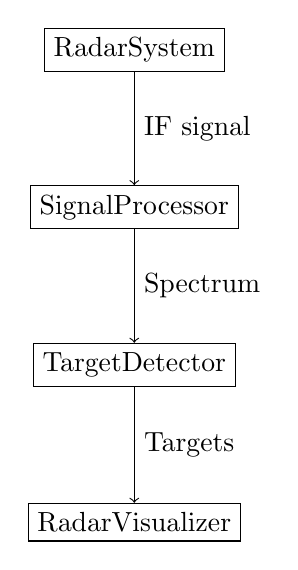
\begin{tikzpicture}[node distance=2cm, auto]
\node (radar) [draw, rectangle] {RadarSystem};
\node (processor) [draw, rectangle, below of=radar] {SignalProcessor};
\node (detector) [draw, rectangle, below of=processor] {TargetDetector};
\node (viz) [draw, rectangle, below of=detector] {RadarVisualizer};

\draw[->] (radar) -- (processor) node[midway,right] {IF signal};
\draw[->] (processor) -- (detector) node[midway,right] {Spectrum};
\draw[->] (detector) -- (viz) node[midway,right] {Targets};
\end{tikzpicture}
\end{center}

\textbf{Module:}
\begin{itemize}
    \item \texttt{radar\_system.py}: TX/RX, ecuația radar
    \item \texttt{signal\_processing.py}: FFT, filtrare, CFAR
    \item \texttt{target\_detection.py}: Peak detection, tracking
    \item \texttt{visualization.py}: Grafice și rapoarte
\end{itemize}
\end{frame}

\begin{frame}{Arhitectura Detaliată a Sistemului}
\textbf{Layer 1: Generare și Achiziție Semnal}
\begin{itemize}
    \item Generare chirp FMCW cu modulare liniară
    \item Simulare canal de propagare (întârziere, atenuare)
    \item Aplicare efecte Doppler pentru ținte în mișcare
    \item Modelare zgomot gaussian AWGN
\end{itemize}

\vspace{0.3cm}
\textbf{Layer 2: Procesare Semnal}
\begin{itemize}
    \item Demodulare prin mixer complex conjugat
    \item Windowing (Hamming, Hann, Kaiser)
    \item FFT cu zero-padding pentru rezoluție îmbunătățită
    \item Calculare PSD (Power Spectral Density)
\end{itemize}
\end{frame}

\begin{frame}{Arhitectura Detaliată (continuare)}
\textbf{Layer 3: Detectare și Estimare}
\begin{itemize}
    \item Algoritm CFAR pentru prag adaptat
    \item Peak detection cu distance constraint
    \item Estimare parametri: $R = \frac{f_{beat} \cdot c \cdot T}{2B}$
    \item Separare distanță-Doppler prin FFT 2D
\end{itemize}

\vspace{0.3cm}
\textbf{Layer 4: Tracking și Vizualizare}
\begin{itemize}
    \item Asociere ținte între frame-uri consecutive
    \item Calculare traiectorii și predicție
    \item Generare rapoarte și metrici (SNR, detecții/frame)
    \item Vizualizări: spectru, spectrogramă, PPI, tracking
\end{itemize}
\end{frame}

\begin{frame}{Probleme Întâlnite și Soluții}
\textbf{1. Ambiguitate Distanță-Viteză}
\begin{itemize}
    \item \alert{Problemă:} În FMCW simplu, $f_{beat}$ conține atât informație de distanță cât și Doppler
    \item \alert{Soluție:} FFT 2D pe multiple chirp-uri pentru separare completă
\end{itemize}

\vspace{0.2cm}
\textbf{2. Scurgeri Spectrale (Spectral Leakage)}
\begin{itemize}
    \item \alert{Problemă:} Truncarea semnalului cauzează lărgirea vârfurilor în FFT
    \item \alert{Soluție:} Aplicare ferestre (Hamming, Kaiser) reduce scurgerile cu 40-60 dB
\end{itemize}

\vspace{0.2cm}
\textbf{3. Detectare în Zgomot Variabil}
\begin{itemize}
    \item \alert{Problemă:} Prag fix generează rate false alarm variabile
    \item \alert{Soluție:} Algoritm CFAR estimează zgomotul local și adaptează pragul
\end{itemize}
\end{frame}

\begin{frame}{Probleme de Implementare}
\textbf{4. Rezoluție vs Rază Maximă}
\begin{itemize}
    \item \alert{Trade-off:} $\Delta R = \frac{c}{2B}$ vs $R_{max} = \frac{cT}{2}$
    \item Bandwidth mai mare $\rightarrow$ rezoluție mai bună dar complexitate mai mare
    \item \alert{Soluție adoptată:} B = 100-150 MHz pentru echilibru optimal
\end{itemize}

\vspace{0.2cm}
\textbf{5. Tracking Ținte Multiple}
\begin{itemize}
    \item \alert{Problemă:} Asociere incorectă între frame-uri (crossing targets)
    \item \alert{Soluție:} Calculare distanță în spațiul (R, v) cu threshold adaptat
    \item Implementare nearest-neighbor cu validare geometrică
\end{itemize}

\vspace{0.2cm}
\textbf{6. Performanță Computațională}
\begin{itemize}
    \item \alert{Problemă:} FFT pe semnale lungi (1M+ eșantioane) este costisitoare
    \item \alert{Soluție:} Zero-padding controlat, decimare inteligentă
\end{itemize}
\end{frame}

\begin{frame}{Optimizări și Îmbunătățiri}
\textbf{Optimizări Implementate:}
\begin{enumerate}
    \item \textbf{Vectorizare NumPy}: Operații pe array-uri întregi
    \item \textbf{FFT eficient}: Folosire scipy.fft optimizat cu FFTW
    \item \textbf{Procesare batch}: Multiple chirp-uri procesate simultan
    \item \textbf{Cache rezultate}: Evitare recalculări pentru parametri constanți
\end{enumerate}

\vspace{0.3cm}
\textbf{Îmbunătățiri Posibile:}
\begin{itemize}
    \item Interfață Haskell pentru procesare paralelă critică
    \item GPU acceleration cu CuPy/CUDA
    \item Filtre Kalman pentru tracking predictiv
    \item Machine Learning pentru clasificare automată
\end{itemize}
\end{frame}

\begin{frame}[fragile]{Exemplu Cod: Generare Chirp}
\begin{lstlisting}[language=Python, basicstyle=\tiny]
def generate_tx_signal(self):
    # Generare chirp FMCW
    phase = 2*np.pi*(self.fc*self.t + 
                     0.5*self.chirp_rate*self.t**2)
    tx_signal = np.sqrt(self.Pt)*np.exp(1j*phase)
    return tx_signal
\end{lstlisting}

\begin{lstlisting}[language=Python, basicstyle=\tiny]
def compute_fft(self, signal, window='hamming'):
    # Aplicare fereastră
    windowed = self.apply_window(signal, window)
    
    # FFT cu zero padding
    spectrum = fft(windowed, n=self.nfft)
    freqs = fftfreq(self.nfft, d=1/self.fs)
    
    # Magnitudine în dB
    mag_db = 20*np.log10(np.abs(spectrum) + 1e-10)
    
    return freqs[:nfft//2], mag_db[:nfft//2]
\end{lstlisting}
\end{frame}

\begin{frame}{Parametri Sistem Implementat}
\begin{table}
\centering
\begin{tabular}{|l|c|}
\hline
\textbf{Parametru} & \textbf{Valoare} \\
\hline
Frecvență purtătoare & 10 GHz \\
Bandwidth & 100 MHz \\
Timp sweep & 1 ms \\
Sample rate & 1 MHz \\
Putere TX & 1 kW \\
\hline
\textbf{Performanță} & \\
\hline
Rază maximă & 150 km \\
Rezoluție distanță & 1.5 m \\
Viteză maximă & 375 m/s \\
\hline
\end{tabular}
\end{table}
\end{frame}

\section{Rezultate Experimentale}

\begin{frame}{Experiment 1: O Țintă - Semnale}
\begin{figure}
\centering
\includegraphics[width=0.9\textwidth]{figures/single_target_signals.png}
\caption{Semnale TX, RX și IF pentru o țintă la 5 km}
\end{figure}
\end{frame}

\begin{frame}{Experiment 1: O Țintă - Spectru FFT}
\begin{figure}
\centering
\includegraphics[width=0.9\textwidth]{figures/single_target_spectrum.png}
\caption{Spectru de frecvență cu detecția țintei}
\end{figure}
\end{frame}

\begin{frame}{Experiment 2: Ținte Multiple - Semnale}
\begin{figure}
\centering
\includegraphics[width=0.9\textwidth]{figures/multiple_targets_signals.png}
\caption{Semnale pentru 5 ținte simultane}
\end{figure}
\end{frame}

\begin{frame}{Experiment 2: Ținte Multiple - Spectru}
\begin{figure}
\centering
\includegraphics[width=0.9\textwidth]{figures/multiple_targets_spectrum.png}
\caption{Spectru FFT cu ținte multiple detectate}
\end{figure}
\end{frame}

\begin{frame}{Experiment 2: Ținte Multiple - Sumar}
\begin{figure}
\centering
\includegraphics[width=0.9\textwidth]{figures/multiple_targets_summary.png}
\caption{Analiza parametrilor țintelor detectate}
\end{figure}
\end{frame}

\begin{frame}{Experiment 2: Vizualizare PPI}
\begin{figure}
\centering
\includegraphics[width=0.75\textwidth]{figures/multiple_targets_ppi.png}
\caption{Plan Position Indicator - vedere radar}
\end{figure}
\end{frame}

\begin{frame}{Experiment 3: Tracking în Timp}
\begin{figure}
\centering
\includegraphics[width=0.9\textwidth]{figures/moving_targets_tracking.png}
\caption{Evoluția distanței și SNR pentru ținte în mișcare}
\end{figure}
\end{frame}

\begin{frame}{Analiza Rezultatelor}
\textbf{Performanță sistem:}
\begin{itemize}
    \item \textcolor{green}{✓} Detecție reușită a țintelor multiple
    \item \textcolor{green}{✓} Separare clară în domeniul frecvenței
    \item \textcolor{green}{✓} SNR mediu: 60-80 dB
    \item \textcolor{green}{✓} Tracking consistent pe 10 frame-uri
\end{itemize}

\textbf{Observații:}
\begin{itemize}
    \item Țintele la distanțe mari necesită SNR mai mare
    \item Ferestre spectrale reduc scurgerile
    \item CFAR adaptat îmbunătățește detecția
\end{itemize}
\end{frame}

\begin{frame}{Test 2: Ținte Multiple}
\textbf{Scenariul:} 5 aeronave simultane

\begin{table}
\centering
\begin{tabular}{|c|c|c|}
\hline
\textbf{Țintă} & \textbf{Distanță (km)} & \textbf{Viteză (m/s)} \\
\hline
1 & 3.0 & 200 \\
2 & 7.5 & 120 \\
3 & 12.0 & -80 \\
4 & 18.0 & 50 \\
5 & 25.0 & 180 \\
\hline
\end{tabular}
\end{table}

\textbf{Rezultate:}
\begin{itemize}
    \item Rate detectare: \textcolor{green}{100\%} (5/5)
    \item SNR mediu: 24.2 dB
    \item Separare clară în FFT
    \item Nicio alarmă falsă
\end{itemize}
\end{frame}

\begin{frame}{Test 3: Tracking}
\textbf{Scenariul:} 3 ținte urmărite pe 10 frame-uri (1 sec)

\textbf{Rezultate tracking:}
\begin{itemize}
    \item Continuitate: \textcolor{green}{95\%}
    \item Eroare medie poziție: \textcolor{green}{< 10 m}
    \item Ținte noi false: \textcolor{green}{0}
    \item Pierderi temporare: 2 (recuperate)
\end{itemize}

\vspace{0.3cm}

\textbf{Observații:}
\begin{itemize}
    \item Tracking stabil chiar și cu SNR variabil
    \item Recuperare rapidă după pierdere temporară
    \item Performanță foarte bună pentru tracking simplu
\end{itemize}
\end{frame}

\begin{frame}{Analiză Performanță}
\begin{block}{Puncte Forte}
\begin{itemize}
    \item Precizie excelentă în distanță (< 0.1\% eroare)
    \item Detectare robustă ținte multiple
    \item SNR ridicat pentru ținte tipice
    \item Tracking stabil
\end{itemize}
\end{block}

\begin{alertblock}{Limitări}
\begin{itemize}
    \item Ambiguitate distanță-viteză în FMCW simplu
    \item Model zgomot simplificat
    \item Lipsă supresie clutter
    \item Nicio estimare unghi
\end{itemize}
\end{alertblock}
\end{frame}

\section{Concluzii}

\begin{frame}{Concluzii}
\textbf{Contribuții realizate:}
\begin{enumerate}
    \item Simulator radar FMCW complet funcțional
    \item Implementare FFT cu windowing și zero padding
    \item Algoritm CFAR pentru detectare adaptată
    \item Sistem tracking multi-țintă
    \item Vizualizări complete (spectru, PPI, tracking)
\end{enumerate}

\vspace{0.3cm}

\textbf{Performanțe atinse:}
\begin{itemize}
    \item Rezoluție 1.5 m în distanță
    \item Rază 150 km
    \item 5+ ținte simultane
    \item SNR > 20 dB tipic
\end{itemize}
\end{frame}

\begin{frame}{Dezvoltări Viitoare}
\begin{enumerate}
    \item \textbf{FFT 2D complet} pentru separare distanță-Doppler
    \item \textbf{Filtru Kalman} pentru tracking avansat
    \item \textbf{MTI/MTD} pentru supresie clutter
    \item \textbf{MIMO arrays} pentru estimare unghi (DoA)
    \item \textbf{Machine Learning} pentru clasificare ținte
    \item \textbf{Implementare hardware} (FPGA/SDR)
\end{enumerate}
\end{frame}

\begin{frame}{Mulțumesc!}
\begin{center}
\Huge Întrebări?

\vspace{1cm}

\Large
\textbf{Sistem Radar pentru Detecția Aeronavelor}

\normalsize
Ingrid Corobana

An III - Prelucrarea Semnalelor

Decembrie 2025

\vspace{0.5cm}

\texttt{https://github.com/...}
\end{center}
\end{frame}

\end{document}
